\documentclass[10pt,twocolumn,letterpaper]{article}

\usepackage{cvpr}
\usepackage{times}
\usepackage{epsfig}
\usepackage{graphicx}
\usepackage{amsmath}
\usepackage{amssymb}

% Include other packages here, before hyperref.

% If you comment hyperref and then uncomment it, you should delete
% egpaper.aux before re-running latex.  (Or just hit 'q' on the first latex
% run, let it finish, and you should be clear).
\usepackage[pagebackref=true,breaklinks=true,letterpaper=true,colorlinks,bookmarks=false]{hyperref}

 \cvprfinalcopy % *** Uncomment this line for the final submission

\def\cvprPaperID{****} % *** Enter the CVPR Paper ID here
\def\httilde{\mbox{\tt\raisebox{-.5ex}{\symbol{126}}}}

% Pages are numbered in submission mode, and unnumbered in camera-ready
\ifcvprfinal\pagestyle{empty}\fi
\begin{document}

%%%%%%%%% TITLE
\title{Improving Millimeter Wave Radar Perception with Deep Learning}

\author{Junfeng Guan \hspace{2cm} Sohrab Madani\\
ECE 544 Project Proposal\\
{\tt\small jguan8@illinois.edu  \hspace{2cm} smadani2@illinois.edu}
% For a paper whose authors are all at the same institution,
% omit the following lines up until the closing ``}''.
% Additional authors and addresses can be added with ``\and'',
% just like the second author.
% To save space, use either the email address or home page, not both
}

\maketitle
%\thispagestyle{empty}

%%%%%%%%% BODY TEXT
\section{Introduction and Project Descriptions}
Nowadays, AI and deep learning play an essential role in the emerging industry of self-driving cars. They are widely applied on sensor data to localize and map objects, as well as for scene-understanding. Previous works have demonstrated precise and accurate perception in most scenarios. However, most of the previous work is limited to data obtained from sensors like LiDAR and cameras, which rely on optical frequencies. As a result, their image quality deteriorates significantly in low visibility conditions such as fog, smog, and snowstorms. This limitation in severe weather conditions is going to be a major roadblock to achieving the vision of full autonomy for vehicles. 

In contrast, RF signals have the advantage that they have more favorable penetration properties, and can hence provide an alternate imaging solution in such inclement weather. The advent of Millimeter-Wave technology provides a good candidate for such RF imaging since along with good propagation characteristics, it also provides huge bandwidth and large-aperture antenna arrays. This enables accurate Time-of-Flight (ToF) and Angle-of-Arrival (AoA) estimation for imaging. However, the imaging resolution in Millimeter-Wave is still not high enough to allow for applications like object detection or scene-understanding. Moreover, with RF one faces the issue of specularity, where reflections from objects may not come back to the receiver depending on the angle of incidence of the transmitted signal. Due to these challenges, the current state-of-the-art in autonomous vehicles uses mmWave radars only for forward ranging to detect the distance from the car ahead, instead of using it for imaging. 

In this project, we propose to develop techniques that can enable high resolution imaging in low visibility conditions with RF signals. Our goal is to use deep learning models to enhance the low resolution images obtained from Millimeter wave radars, and enable various crucial vision applications for autonomous vehicles like lane detection, image mapping, localization, and object identification.


%  In contrast, radar has more favorable propagation characteristics in such inclement weather, due to its better penetration properties. Traditional radar imaging resolution is not comparable with that from LiDAR. The rising of Millimeter-Wave (mmWave) and 5G technology offers more accurate Time-of-Flight (ToF) and Angle-of-Arrival (AoA) estimation, because of the wider available bandwidth and miniature size antenna arrays. However, LiDAR performance still exceeds that of Millimeter-wave radar.
%\par In this project, we are looking forward to investigating the possibility of improving Millimeter wave radar imaging resolution by applying deep learning. 

\section{Proposed Method}
Millimeter radars transmitter shines a radar waveform, which gets reflected by objects, and the reflected waveform will be received by the receiver. Comparing the transmitted and received radar signal, we can measure Time-of-Flight (ToF), which suggests the round-trip distance between radar and reflectors. Besides, with an array of radar receivers, we can also extract the Direction-of-Arrival (DoA) of the reflected waves. Knowing the distance and angle of reflectors in the space, we can localize them in a polar coordinate. 

\par Due to the resolution limit, every pixel in radar images may correspond to a combination of many nearby point reflectors within the distance and angular bin. Therefore, low resolution radar images appear less informative to human. However, this combination of reflection should still follow certain pattern and can be analyzed to distinguish and infer features of the target object. Especially in the application of self-driving cars, we are mostly interested in vehicle and human targets. They both have very unique shapes and motion patterns. If we train our neural network with the combined reflection from point reflectors with certain distribution, we should be able to classify and map the low resolution pixels to the actually shape of the target. Besides, the specularity of RF prevent us from receiving reflection from all features of the target object, and neural networks can help us infer the shape and location of the entire target by analyzing a time series of incomplete images of the object. For example, if we can pin point the head, chest and legs of a person along the trace of the object motion, we can fill up the rest parts of him in our map. 
 
\par RF-Pose3D ~\cite{rfpose} ~\cite{rfpose3D} demonstrates Convolutional Neural Network (CNN) that can recreate the human body skeletons by tracking 14 key points. Because CNNs leverage local dependencies in the data, it significantly reduces the total number of weights to be learned. Considering this favorable property of CNN, we are going to implement this model first in our project. In contrast, we will concentrate more on classifying features of vehicles to infer the shape, orientation, and even velocity. We are planning to start with 2D images, which contains the distance and angle of objects within a horizontal plane, then we will try to extend to 3D images.

\section{Dataset Description}
The dataset we will create should include all significant features of a car. Therefore, we will place a car in a number of orientations in front of the radar, and try to filter out noise and interferences from other key points in preprocessing. We will also simulate the most likely relative positions and motions of the autonomous car with the radar system and other vehicles on the road, take a series of images as they move together.
\par We might have to face the problem of lack of accurate labels to our training set. One possible solution is to collect another set of reference data with cameras and train an additional neural network with well-developed vision models to label our radar images.

\section{Proposed Experiments}
We will conduct outdoor experiments on the top floor of the parking garage. Radar images (both 2D and 3D) will be collected with our custom-built Millimeter wave FMCW (Frequency Modulated Continuous Wave) radar system, operating around 60 GHz as shown in the figure above Both the radar transmitter and receiver antennas will be omni-directional. While the transmitter remains fixed, the receiver will move on a linear stage to synthesize a 1D or 2D antenna array to obtain the Direction of Arrival (DoA) measurement in a horizontal plane or the entire 3D space. We will first process raw radar data with fundamental radar signal processing algorithms, and filter out noise and unwanted interference to focus on only a few key features of the target. The target of interest can be either static or under motion. 

\begin{figure}
\centering
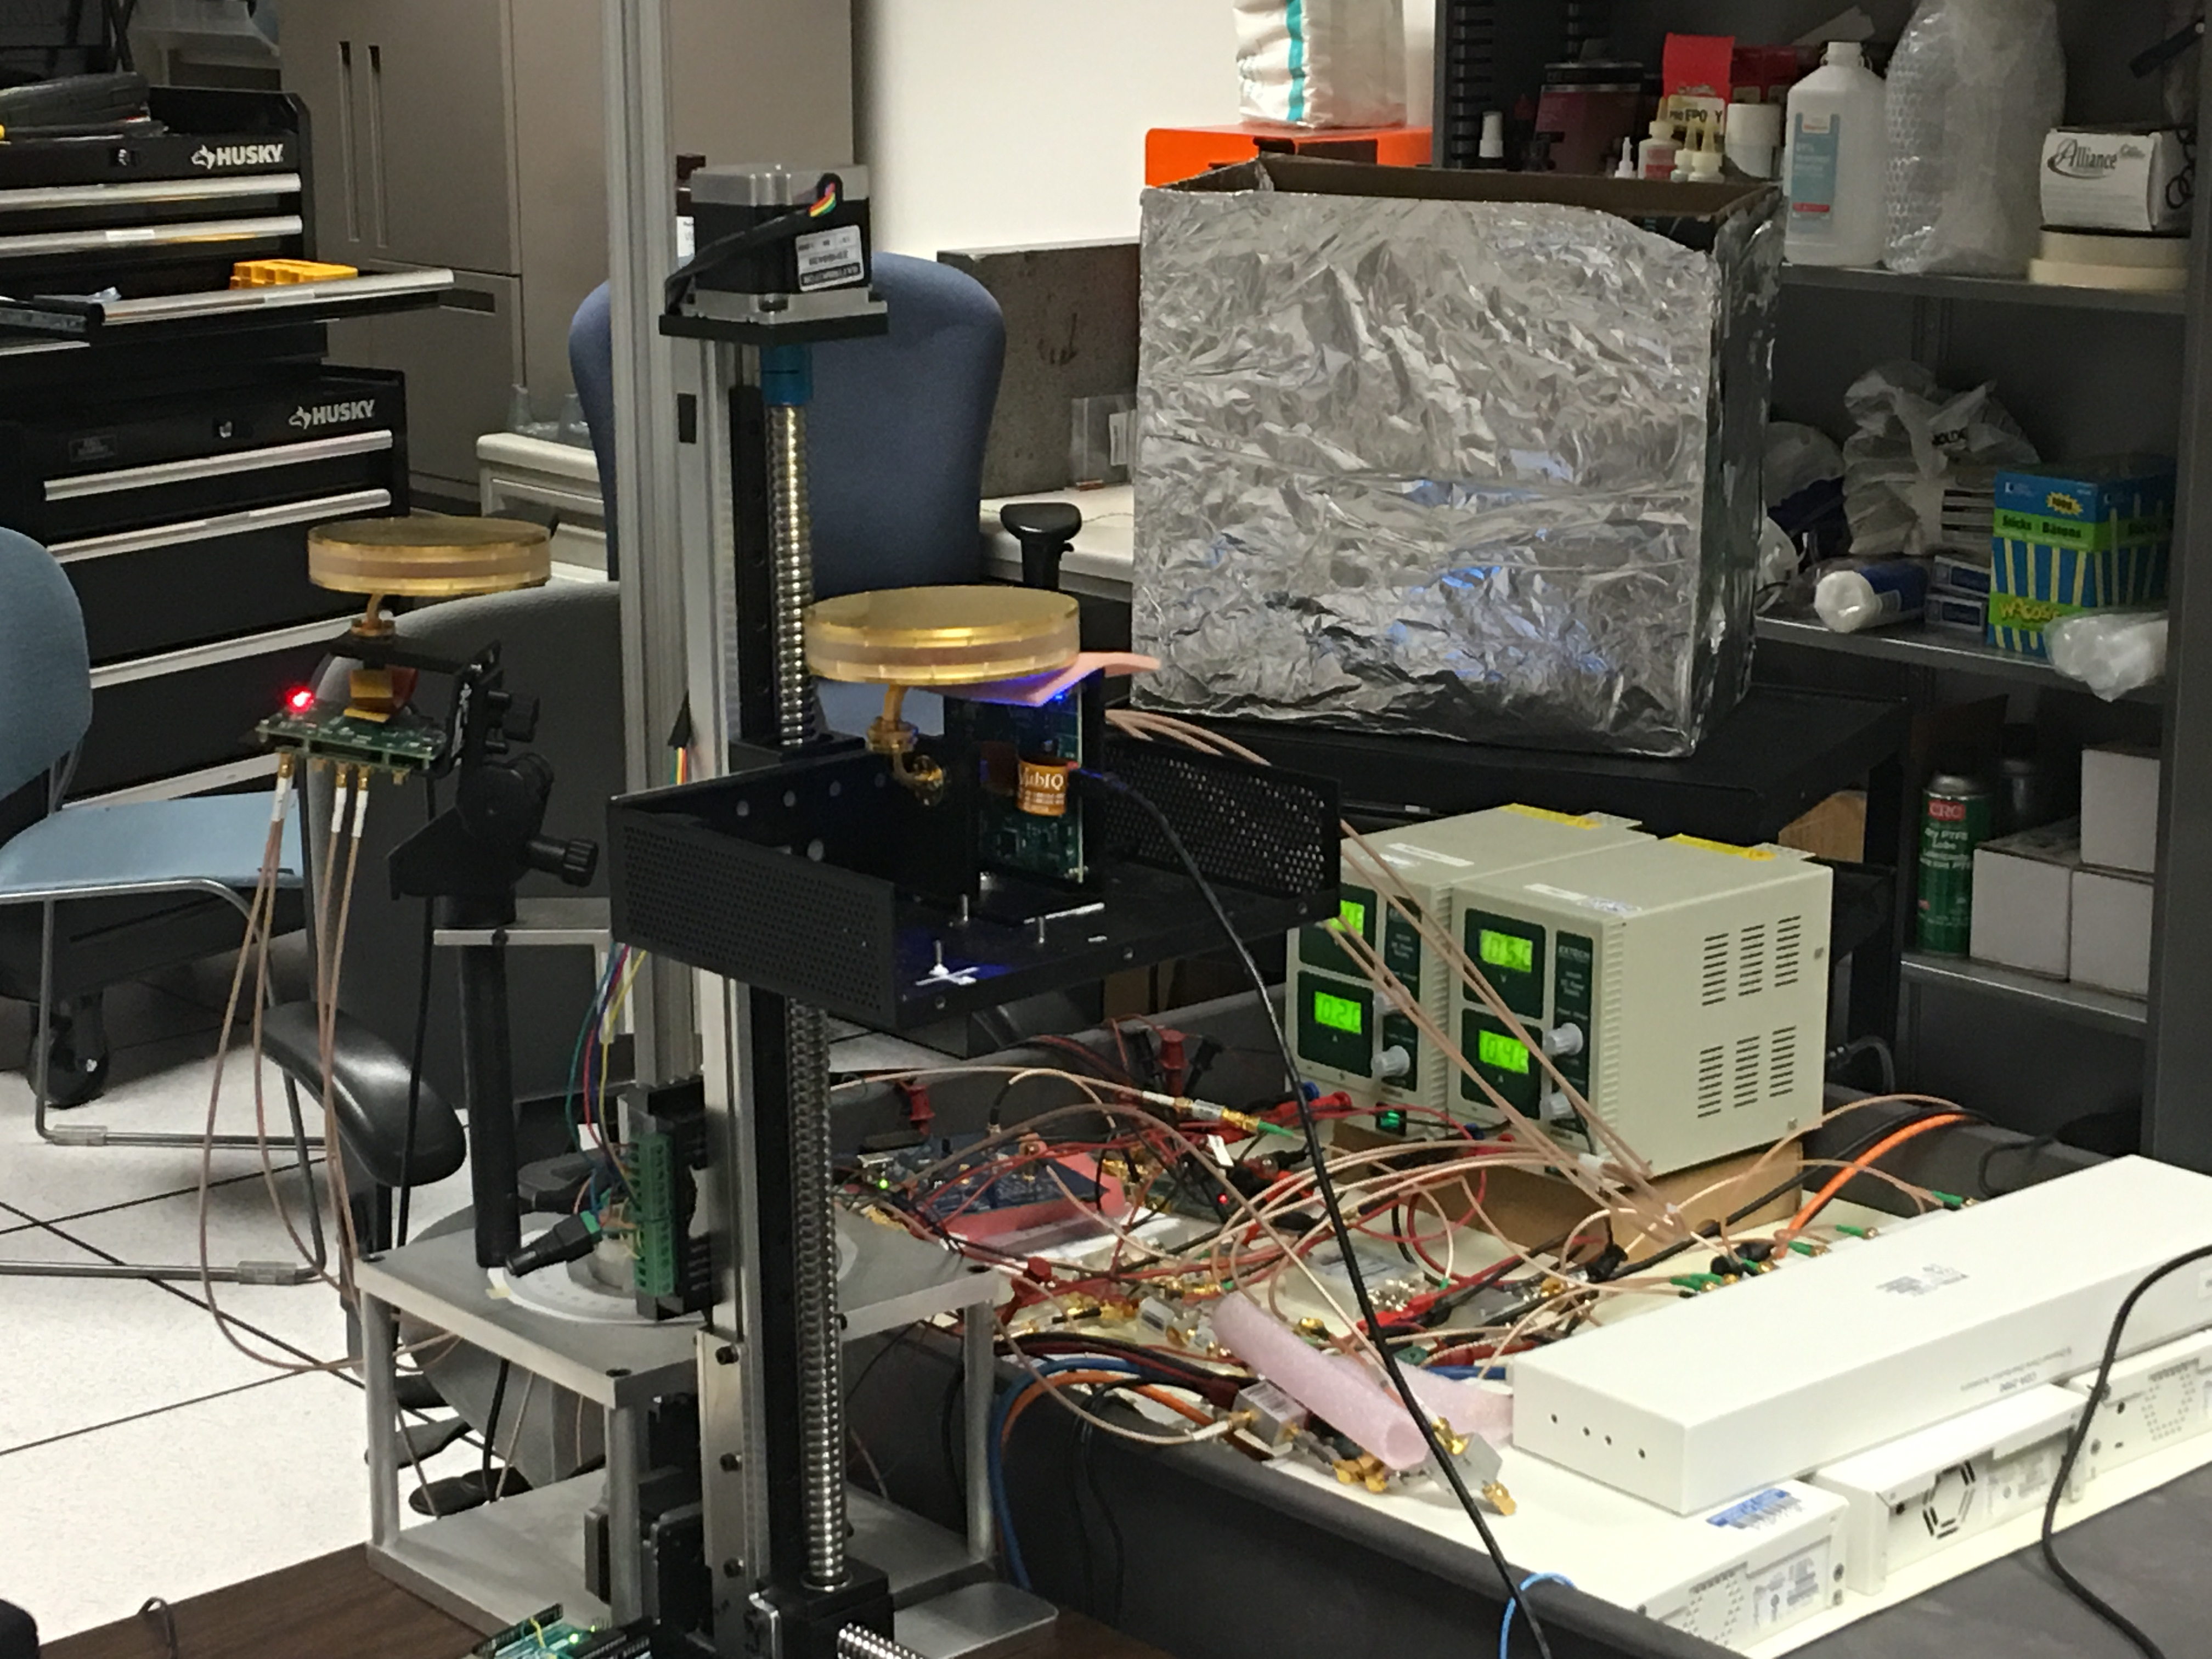
\includegraphics[width=8cm,height=6cm]{./figure/experiment_setup.jpg}
\caption{Custom-built 60 GHz mmWave radar imaging system}
\end{figure}

\section{Resource Feasibility}
We already have a working radar imaging system, and there are cars and space available for us to create the training dataset. Besides, we also have access to the campus cluster for neural network training, so there should not be any major resource limits for our project.

\section{Tentative timeline and the necessary steps}

This project can be roughly divided into three stages:\\
1. Creating datasets of 2D and 3D radar images \\
2. Labeling convolutional Neural Network (CNN) training\\
3. Convolutional Neural Network (CNN) training on 2D radar images\\
4. Convolutional Neural Network (CNN) training on 3D radar images\\
The detailed steps and timeline are shown in the table above.

\begin{table}[]
	\begin{tabular}{|c|c|}
		\hline
		Step & Deadline \\ \hline
		Create 2D static dataset  &  10/9 \\ \hline
		Train labeling neural network & 10/16 \\ \hline
	    Create 2D dynamic dataset & 10/16 \\ \hline
	    Build 2D imaging CNN & 10/23 \\ \hline
	    Train 2D imaging CNN & 10/30 \\ \hline
	    Evaluate 2D imaging CNN & 11/6 \\ \hline
		Create 3D static dataset  & 11/13 \\ \hline
		Create 3D dynamic dataset & 11/13 \\ \hline
		Build 2D imaging CNN & 11/20 \\ \hline
		Train 2D imaging CNN & 11/27 \\ \hline
		Evaluate 2D imaging CNN & 12/4 \\ \hline
		Report writing & 12/17 \\ \hline
	\end{tabular}
	\caption{Steps and timeline}
\end{table}

\begin{thebibliography}{999}
	\bibitem{rfpose}
		M. Zhao, T. Li, M. A. Alsheikh, Y. Tian, H. Zhao, A. Torralba, and D. Katabi,
		Trhough-Wall Human Pose Estimation Using Radio Signals,
		IEEE Conference on Computer Vision and Pattern Recognition, CVPR, 2018.
	\bibitem{rfpose3D}
		M. Zhao, Y. Tian, H. Zhao, M. A. Alsheikh, T. Li, R. Hristov, Zachary Kabelac, D. Katabi, A. Torralba,
		RF-Based 3D Skeletons, SIGCOMM, 2018.

\end{thebibliography}

\end{document}
